% A LaTeX template for MSc Thesis submissions to 
% Politecnico di Milano (PoliMi) - School of Industrial and Information Engineering
%
% S. Bonetti, A. Gruttadauria, G. Mescolini, A. Zingaro
% e-mail: template-tesi-ingind@polimi.it
%
% Last Revision: October 2021
%
% Copyright 2021 Politecnico di Milano, Italy. NC-BY

\documentclass{Configuration_Files/PoliMi3i_thesis}
%------------------------------------------------------------------------------
%	REQUIRED PACKAGES AND  CONFIGURATIONS
%------------------------------------------------------------------------------

% CONFIGURATIONS
\usepackage{parskip} % For paragraph layout
\usepackage{setspace} % For using single or double spacing
\usepackage{emptypage} % To insert empty pages
\usepackage{multicol} % To write in multiple columns (executive summary)
\setlength\columnsep{15pt} % Column separation in executive summary
\setlength\parindent{0pt} % Indentation
\raggedbottom  

% PACKAGES FOR TITLES
\usepackage{titlesec}
% \titlespacing{\section}{left spacing}{before spacing}{after spacing}
\titlespacing{\section}{0pt}{3.3ex}{2ex}
\titlespacing{\subsection}{0pt}{3.3ex}{1.65ex}
\titlespacing{\subsubsection}{0pt}{3.3ex}{1ex}
\usepackage{color}

% PACKAGES FOR LANGUAGE AND FONT
\usepackage[english]{babel} % The document is in English  
\usepackage[utf8x]{inputenc} % UTF8 encoding
\usepackage[T1]{fontenc} % Font encoding
\usepackage[11pt]{moresize} % Big fonts

% PACKAGES FOR IMAGES
\usepackage{graphicx}
\usepackage{transparent} % Enables transparent images
\usepackage{eso-pic} % For the background picture on the title page
\usepackage{subfig} % Numbered and caption subfigures using \subfloat.
\usepackage{tikz} % A package for high-quality hand-made figures.
\usetikzlibrary{}
\graphicspath{{./Images/}} % Directory of the images
\usepackage{caption} % Coloured captions
\usepackage{xcolor} % Coloured captions
\usepackage{amsthm,thmtools,xcolor} % Coloured "Theorem"
\usepackage{float}

% STANDARD MATH PACKAGES
\usepackage{amsmath}
\usepackage{amsthm}
\usepackage{amssymb}
\usepackage{amsfonts}
\usepackage{bm}
\usepackage[overload]{empheq} % For braced-style systems of equations.
\usepackage{fix-cm} % To override original LaTeX restrictions on sizes

% PACKAGES FOR TABLES
\usepackage{tabularx}
\usepackage{longtable} % Tables that can span several pages
\usepackage{colortbl}

% PACKAGES FOR ALGORITHMS (PSEUDO-CODE)
\usepackage{algorithm}
\usepackage{algorithmic}


% PACKAGES FOR REFERENCES & BIBLIOGRAPHY
%\usepackage[colorlinks=true,linkcolor=black,anchorcolor=black,citecolor=black,filecolor=black,menucolor=black,runcolor=black,urlcolor=black]{hyperref} % Adds clickable links at references
%\usepackage{cleveref}
%\usepackage[square, numbers, sort&compress]{natbib} % Square brackets, citing references with numbers, citations sorted by appearance in the text and compressed
%\bibliographystyle{siam} % You may use a different style adapted to your field

% PACKAGES FOR REFERENCES & BIBLIOGRAPHY
\usepackage[colorlinks=true,linkcolor=black,anchorcolor=black,citecolor=black,filecolor=black,menucolor=black,runcolor=black,urlcolor=black]{hyperref} % Adds clickable links at references
\usepackage{cleveref}
\usepackage[square, numbers, sort&compress]{natbib} % Square brackets, citing references with numbers, citations sorted by appearance in the text and compressed
\bibliographystyle{abbrvnat} % You may use a different style adapted to your field


% OTHER PACKAGES
\usepackage{pdfpages} % To include a pdf file
\usepackage{afterpage}
\usepackage{lipsum} % DUMMY PACKAGE
\usepackage{fancyhdr} % For the headers
\fancyhf{}
\usepackage{eurosym}

% Input of configuration file. Do not change config.tex file unless you really know what you are doing. 
% Define blue color typical of polimi
\definecolor{bluepoli}{cmyk}{0.4,0.1,0,0.4}

% Custom theorem environments
\declaretheoremstyle[
  headfont=\color{bluepoli}\normalfont\bfseries,
  bodyfont=\color{black}\normalfont\itshape,
]{colored}

% Set-up caption colors
\captionsetup[figure]{labelfont={color=bluepoli}} % Set colour of the captions
\captionsetup[table]{labelfont={color=bluepoli}} % Set colour of the captions
%\captionsetup[algorithm]{labelfont={color=bluepoli}} % Set colour of the captions

\theoremstyle{colored}
\newtheorem{theorem}{Theorem}[chapter]
\newtheorem{proposition}{Proposition}[chapter]

% Enhances the features of the standard "table" and "tabular" environments.
\newcommand\T{\rule{0pt}{2.6ex}}
\newcommand\B{\rule[-1.2ex]{0pt}{0pt}}

% Pseudo-code algorithm descriptions.
%\newcounter{algsubstate}
%\renewcommand{\thealgsubstate}{\alph{algsubstate}}
%\newenvironment{algsubstates}
 % {\setcounter{algsubstate}{0}%
  % \renewcommand{\STATE}{%
   %  \stepcounter{algsubstate}%
    % \Statex {\small\thealgsubstate:}\space}}
  %{}

% New font size
\newcommand\numfontsize{\@setfontsize\Huge{200}{60}}

% Title format: chapter
\titleformat{\chapter}[hang]{
\fontsize{50}{20}\selectfont\bfseries\filright}{\textcolor{bluepoli} \thechapter\hsp\hspace{2mm}\textcolor{bluepoli}{|   }\hsp}{0pt}{\huge\bfseries \textcolor{bluepoli}
}

% Title format: section
\titleformat{\section}
{\color{bluepoli}\normalfont\Large\bfseries}
{\color{bluepoli}\thesection.}{1em}{}

% Title format: subsection
\titleformat{\subsection}
{\color{bluepoli}\normalfont\large\bfseries}
{\color{bluepoli}\thesubsection.}{1em}{}

% Title format: subsubsection
\titleformat{\subsubsection}
{\color{bluepoli}\normalfont\large\bfseries}
{\color{bluepoli}\thesubsubsection.}{1em}{}

% Shortening for setting no horizontal-spacing
\newcommand{\hsp}{\hspace{0pt}}

\makeatletter
% Renewcommand: cleardoublepage including the background pic
\renewcommand*\cleardoublepage{%
  \clearpage\if@twoside\ifodd\c@page\else
  \null
  \AddToShipoutPicture*{\BackgroundPic}
  \thispagestyle{empty}%
  \newpage
  \if@twocolumn\hbox{}\newpage\fi\fi\fi}
\makeatother

%For correctly numbering algorithms
%\numberwithin{algorithm}{chapter}

%----------------------------------------------------------------------------
%	NEW COMMANDS DEFINED
%----------------------------------------------------------------------------

% EXAMPLES OF NEW COMMANDS
\newcommand{\bea}{\begin{eqnarray}} % Shortcut for equation arrays
\newcommand{\eea}{\end{eqnarray}}
\newcommand{\e}[1]{\times 10^{#1}}  % Powers of 10 notation

%----------------------------------------------------------------------------
%	ADD YOUR PACKAGES (be careful of package interaction)
%----------------------------------------------------------------------------
%\usepackage{pgfplots}
\usepackage{lscape}
\usepackage{rotating}
\usepackage{lipsum}


%----------------------------------------------------------------------------
%	ADD YOUR DEFINITIONS AND COMMANDS (be careful of existing commands)
%----------------------------------------------------------------------------
\newsavebox{\mybox}
%----------------------------------------------------------------------------
%	BEGIN OF YOUR DOCUMENT
%----------------------------------------------------------------------------




\begin{document}


\fancypagestyle{plain}{%
\fancyhf{} % Clear all header and footer fields
\fancyhead[RO,RE]{\thepage} %RO=right odd, RE=right even
\renewcommand{\headrulewidth}{0pt}
\renewcommand{\footrulewidth}{0pt}}

%----------------------------------------------------------------------------
%	TITLE PAGE
%----------------------------------------------------------------------------

\pagestyle{empty} % No page numbers
\frontmatter % Use roman page numbering style (i, ii, iii, iv...) for the preamble pages

\puttitle{
	title=Local refilling infrastructure for\\ hydrogen or electrical HD fleets, % Title of the thesis
	name= \\ 
	      Alessandro Barbero 10536528 \\
          Luca Cattaneo 10521219 \\
          Mara Pegoraro 10629697 \\
          Jacopo Elia Pometto 10521596 \\
          Giovanni Valtorta 10528573, % Author Name and Surname
	course= Energy and Emissions in transportation systems, % Study Programme (in Italian)
	academicyear={2021-2022},  % Academic Year
} % These info will be put into your Title page 

%----------------------------------------------------------------------------
%	PREAMBLE PAGES: ABSTRACT (inglese e italiano), EXECUTIVE SUMMARY
%----------------------------------------------------------------------------
\startpreamble
\setcounter{page}{1} % Set page counter to 1

% ABSTRACT IN ENGLISH

\chapter*{Abstract} 
The aim of this project work is to provide an answer to the question:

\textit{Could hydrogen be a good solution for substituting fossil fuels in HD transport?}

This question will be answered analysing a case study related to a logistic depot located in northern Italy.

The first part of the report will be devoted to the description of the state of the art of heavy duty transport, the technologies used and the peculiarities of the current circulating fleet.

The subsequent section consists in the presentation of the current solutions used to exploit hydrogen in the energy and transportation sector.

A technical analysis will then be performed, to assess the possibilities and limits of different alternatives to provide the requested hydrogen to the depot, imagining the building of a local refilling infrastructure to respond to the needs of the vehicles that use the depot as a logistic base.

In the end, all those alternatives will be put to the test through an economical evaluation, using as unit of measure the total funds needed to run the refill facility for a year, also taking into consideration the possible $CO_2$ emissions.

The conclusion will present the results in a composite way, providing also an overview of the possible scalability options of the different solutions.

%----------------------------------------------------------------------------
%	LIST OF CONTENTS/FIGURES/TABLES/SYMBOLS
%----------------------------------------------------------------------------

% TABLE OF CONTENTS
\thispagestyle{empty}
\tableofcontents % Table of contents 
\thispagestyle{empty}
\cleardoublepage

%-------------------------------------------------------------------------
%	THESIS MAIN TEXT
%-------------------------------------------------------------------------
% In the main text of your thesis you can write the chapters in two different ways:
%
%(1) As presented in this template you can write:
%    \chapter{Title of the chapter}
%    *body of the chapter*
%
%(2) You can write your chapter in a separated .tex file and then include it in the main file with the following command:
%    \chapter{Title of the chapter}
%    \input{chapter_file.tex}
%
% Especially for long thesis, we recommend you the second option.

%\addtocontents{toc}{\vspace{2em}} % Add a gap in the Contents, for aesthetics
\mainmatter % Begin numeric (1,2,3...) page numbering

% --------------------------------------------------------------------------
% NUMBERED CHAPTERS % Regular chapters following
% --------------------------------------------------------------------------
\newpage
\chapter{Introduction}
Given the report from ACEA\textsuperscript{\cite{ACEA2021}}, we can see that the circulating fleets in EU have an average age of 13 years, with a predominance of diesel powered engine (Figure \ref{fig:hdpower}).
\begin{figure}[hb]
    \centering
    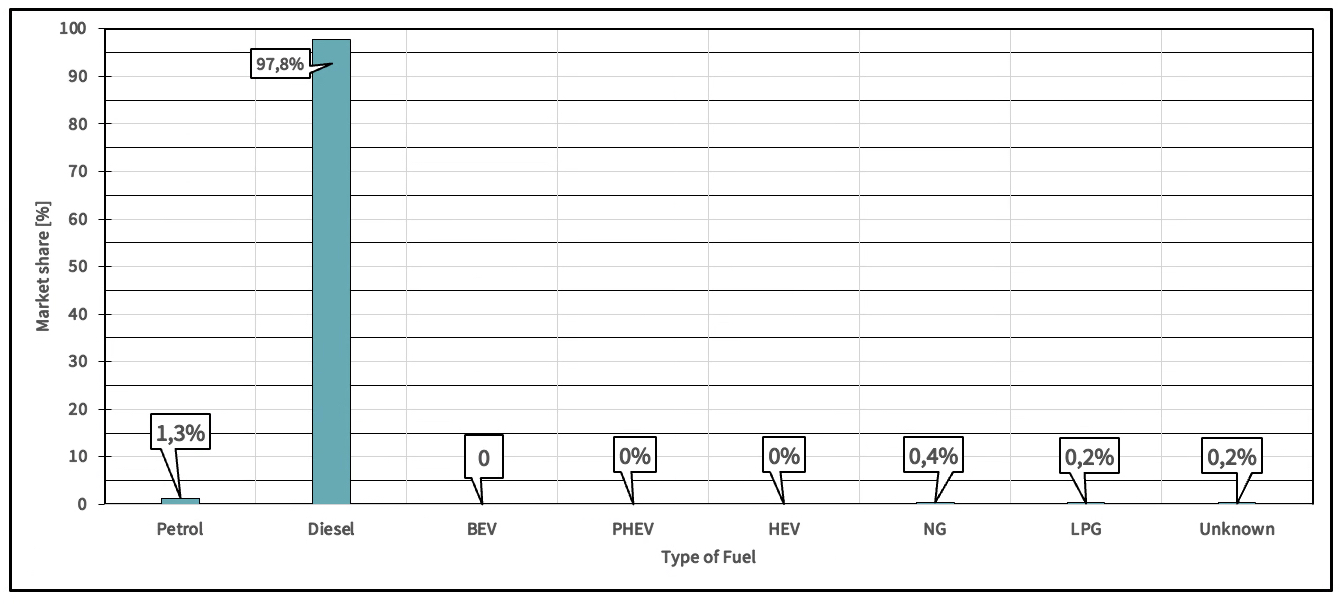
\includegraphics[width=0.7\textwidth]{Chapters/Pictures/Fuels_MarketShare.jpeg}
    \caption{Market share (in percentage) for different types of fuel}
    \label{fig:hdpower}
\end{figure}

So, in compliance with the sustainability goals given by the United Nations, it is necessary to renew also the Heavy Duty sector. In Table \ref{tab:dieselalternative} are shown the main options that can help us reach this objective:

\begin{table}[ht]
\centering
\begin{tabular}{|c|c|c|}
\hline
\rowcolor{bluepoli!40} \multicolumn{1}{|c|}{\textbf{Fuel}} & \multicolumn{1}{c|}{\textbf{PROS}}         & \multicolumn{1}{c|}{\textbf{CONS}} \\ \hline
\textbf{Biofuels} & Derivable from waste products & Still emit $CO_2$ during use \\ \hline
\textbf{Electricity} & \begin{tabular}[c]{@{}c@{}}$100\%$ clean during use; \\ Possible to couple the vehicle \\ with a fixed infrastructure \\ (OVH contact line)\end{tabular} & \begin{tabular}[c]{@{}c@{}}Cleanness depend on energetic mix; \\ Charging infrastructure and time \\ Weight of the battery\end{tabular} \\ \hline
\textbf{Hydrogen} & \begin{tabular}[c]{@{}c@{}}$100\%$ clean during use; \\ Higher energy density\end{tabular} & Lower volumetric density \\ \hline
\end{tabular}
\caption{Pros and Cons of different alternative fuels}
\label{tab:dieselalternative}
\end{table}

As said in a recent book\textsuperscript{\cite{Mazzo2021}}, the use of electric batteries in HD is not so convenient, because of their size and type of use, so we will focus on the $H_2$ technologies and how to produce this hydrogen in a sustainable way.

\section{Sate of the Art}
The field of production of hydrogen is in continuous development and actual technologies are the following\textsuperscript{\cite{guanda20211}}:
\begin{description}
    \item[Oil:] hydrogen is produced with steam reforming or partial oxidation from fossil or renewable oils;
    \item[Gas:] natural or bio-gas are hydrogen sources with steam reforming or partial oxidation;
    \item[Algae:] methods for utilising the photo-synthesis for hydrogen production;
    \item[Wood:] pyrolysis technology for hydrogen from biomass;
    \item[Power:] water electrolysis from renewable sources;
    \item[Coal:] with gasification technology hydrogen may be produced from coal;
    \item[Alcohols:] like hydrogen and methanol derived from gas or biomass (rich in hydrogen and may be reformed to hydrogen).
\end{description}

Due to the physical and geographical characteristics of Italy, we choose to feed the water electrolysis with the power generated by hydropower plant or by photovoltaic plant. This also needed to address the problem of being dependent from the foreign state, such in the case of oil and gas (and to their price fluctuation), that is a theme that started to spread in the last years.

\subsection{Electrolysis}
With electrolysis water is split in hydrogen and oxygen, in an electrochemical cell.

We can made a distinction about the solution based on the cell's temperature\textsuperscript{\cite{guanda20211}}.
\begin{itemize}
    \item Low temperature cells that can be divided into:
    \begin{description}
        \item[Alkaline electrolysis](Figure \ref{fig:alkaline})  based on a liquid solution of $NaOH$ or $KOH$;
        \item[PEM] (Figure \ref{fig:pem}) based on a polymeric electrolyte.
    \end{description}
    \item High temperature cells (such as SOEC).
\end{itemize}

Low temperature cells are already a commercial solution, while high temperature ones are still in development, so we will focus on the first one.

\begin{figure}[hp]
    \centering
    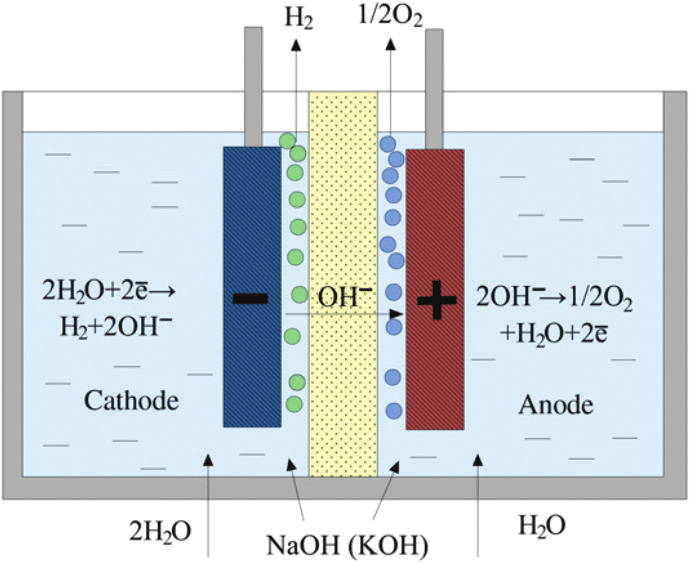
\includegraphics[width=0.5\textwidth]{Chapters/Pictures/Schematic-diagram-of-the-alkaline-electrolysis-cell-34.png}
    \caption{Schematic diagram of the alkaline electrolysis cell.
    (Courtesy of \textbf{\href{https://www.researchgate.net/figure/Schematic-diagram-of-the-alkaline-electrolysis-cell-34_fig4_327179309}{Scientific Figure on ResearchGate}})}
    \label{fig:alkaline}
\end{figure}

\begin{figure}[hp]
    \centering
    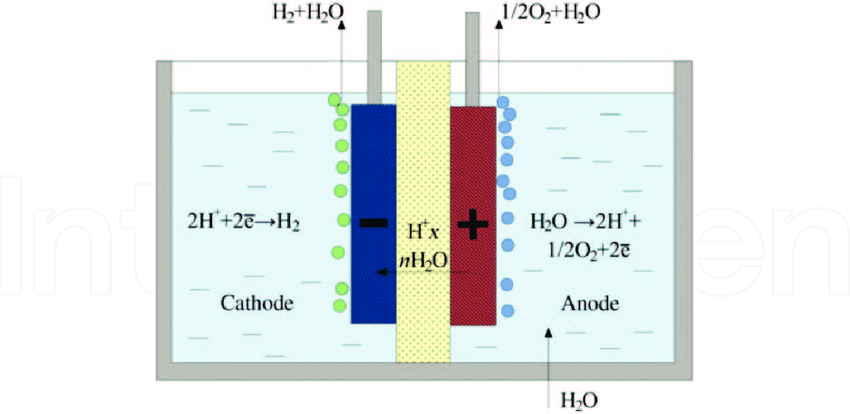
\includegraphics[width=0.8\textwidth]{Chapters/Pictures/Schematic-diagram-of-PEM-electrolysis-cell-33.png}
    \caption{Schematic diagram of PEM electrolysis cell.
    (Courtesy of \textbf{\href{https://www.researchgate.net/figure/Schematic-diagram-of-PEM-electrolysis-cell-33_fig1_327179309}{Scientific Figure on ResearchGate}})}
    \label{fig:pem}
\end{figure}

\subsection{Hydropower}
Hydropower plants use the potential energy of water flowing down to the turbine to produce electrical energy. We can find two main configurations\textsuperscript{\cite{lakohydro2010}}:
\begin{itemize}
    \item dams with reservoirs (Figure \ref{fig:dam}), that can be classified into:
    \begin{itemize}
        \item small dams;
        \item large dams;
        \item pumped storage;
    \end{itemize}
    \item run-of-the-river.
\end{itemize}

This technology does not produce significant $CO_2$ emissions other than those emitted during plants construction. 

It is also a mature technology: many of the plants that were built in the early decades of the $20^{th}$ century are currently still in operation. This reduces the costs of the facilities, because they consist simply in O$\&$M.

\begin{figure}[h]
    \centering
    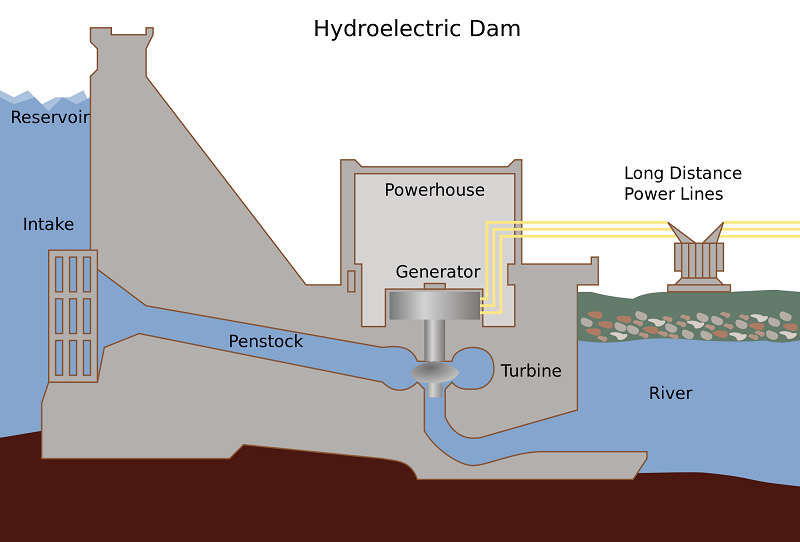
\includegraphics[width=0.6\textwidth]{Chapters/Pictures/Damparts.png}
    \caption{\small{A diagram showing the main components of a conventional hydroelectric facility.
    (Courtesy of \textbf{\href{https://energyeducation.ca/wiki/images/8/8e/Damparts.png}{energy education}})}}
    \label{fig:dam}
\end{figure}

Otherwise hydropower depends on rainfall and a reserve may be needed to compensate for periods of low rainfall. So, it will be possible that climate change influences the efficiency of such technology. We also have to take in account the political, societal and economic risk usual of this type of infrastructures.

\subsection{Photovoltaic}

\Huge{TO DO}
\newpage
\chapter{Case Study Description}
\begin{table}[ht!]
\centering
\begin{tabular}{|lc|}
\hline
\multicolumn{2}{|c|}{\cellcolor{bluepoli!40}{\textbf{Scania G series}}}                       \\ \hline
\multicolumn{1}{|l|}{WLTP Consumption {[}kg/km{]}}                     & $0,066$              \\ \hline
\multicolumn{1}{|l|}{Number of trucks}                                 & $5$                  \\ \hline
\multicolumn{1}{|l|}{Distance {[}km/day{]}}                            & $500$                \\ \hline
\multicolumn{1}{|l|}{Total $H_2$ required {[}kg/day{]}}                & $165$                \\ \hline
\multicolumn{1}{|l|}{LHV $H_2$ {[}kWh/kg{]}}                           & $33,31$              \\ \hline
\multicolumn{1}{|l|}{Electric energy required {[}MWh{]}}               & $8,456$              \\ \hline
\end{tabular}
\caption{Truck data}
\label{tab:truckdata}
\end{table}

\begin{table}[h]
\centering
\begin{tabular}{|lc|}
\hline
\rowcolor{bluepoli!40} \multicolumn{2}{|c|}{\textbf{Hydroelectric PP in Trezzo sull'Adda}}        \\ \hline
\multicolumn{1}{|l|}{Efficient power {[}kW{]}}              & $10.500$                            \\ \hline
\multicolumn{1}{|l|}{Mean produceable energy {[}kWh{]}}     & $65.000.000$                        \\ \hline
\multicolumn{1}{|l|}{$V_{line}$ {[}V{]}}                    & $200.000$                           \\ \hline
\multicolumn{1}{|l|}{$I_{line}$ {[}A{]}}                    & $52,5$                              \\ \hline
\multicolumn{1}{|l|}{Power loss percentage (HV systems)}    & $2\%$                               \\ \hline
\multicolumn{1}{|l|}{Effective power {[}kW{]}}              & $10.290$                            \\ \hline
\rowcolor{bluepoli!40} \multicolumn{2}{|c|}{\textbf{Electrolyzer on site}}                        \\ \hline
\rowcolor{bluepoli!40} \multicolumn{2}{|c|}{\textbf{Cost of transport by truck (gaseous $H_2$)}}  \\ \hline
\multicolumn{1}{|l|}{Unitary cost {[}€/kg{]}}               & $3$                                 \\ \hline
\multicolumn{1}{|l|}{Total cost {[}€{]}}                    & $544,5$                             \\ \hline
\multicolumn{1}{|l|}{Distance from depot {[}km{]}}          & $40$                                \\ \hline
\multicolumn{1}{|l|}{Emissions {[}$g_{CO_2}$/km{]}}         & $94$                                \\ \hline
\multicolumn{1}{|l|}{Total daily $CO_2$ emission}           & $7.520$                             \\ \hline
\end{tabular}
\caption{Hydroelectric power plant and electrolyzer on site}
\label{tab:firstsolution}
\end{table}

\begin{table}[ht]
\centering
\begin{tabular}{|lc|}
\hline
\multicolumn{2}{|c|}{\cellcolor{bluepoli!40}Hydroelectric PP in Crodo}               \\ \hline
\multicolumn{1}{|l|}{Efficient power {[}kW{]}}                      & $52.800$       \\ \hline
\multicolumn{1}{|l|}{Distance from depot {[}km{]}}                  & $160$          \\ \hline
\multicolumn{1}{|l|}{$V_{line}$ {[}V{]}}                            & $200.000$      \\ \hline
\multicolumn{1}{|l|}{$I_{line}$ {[}A{]}}                            & $264$          \\ \hline
\multicolumn{1}{|l|}{Power loss percentage (HV systems)}            & $2\%$          \\ \hline
\multicolumn{1}{|l|}{Effective power {[}kW{]}}                      & $51.744$       \\ \hline
\multicolumn{2}{|c|}{\cellcolor{bluepoli!40}Electrolyzer near the depot}             \\ \hline
\multicolumn{1}{|l|}{$H_2$ request {[}kg/day{]}}                    & $181,50$       \\ \hline
\multicolumn{1}{|l|}{Maximum $H_2$ production {[}kg/h{]}}           & $36$           \\ \hline
\multicolumn{1}{|l|}{Maximum power {[}kW{]}}                        & $2.350$        \\ \hline
\multicolumn{1}{|l|}{Production to satisfy demand in 8h {[}kg/h{]}} & $22,6875$      \\ \hline
\multicolumn{1}{|l|}{Actual required power {[}kW{]}}                & $1480,99$      \\ \hline
\multicolumn{2}{|c|}{\cellcolor{bluepoli!40}Electric grid}                           \\ \hline
\multicolumn{1}{|l|}{Energy required {[}MWh{]}}                     & $11,85$        \\ \hline
\multicolumn{1}{|l|}{EU average energy cost {[}€/kWh{]}}            & $0,02864$      \\ \hline
\multicolumn{1}{|l|}{Total cost {[}€{]}}                            & $339,324$      \\ \hline
\end{tabular}
\caption{Hydroelectric power plant and electrolyzer near the depot}
\label{tab:secondsolution}
\end{table}

\section{Logistic Depot}
\section{Hydro}
\subsection{Near Electrolysis}
\subsection{Far Electrolysis}
\section{Only transport}
\chapter{Technical Evaluation}
We will now describe in detail, for each main case, the different results of the proposed solution. Firstly, we computed the requested energy and hydrogen to run \textbf{10 }trucks per $500$ km/day, as we can see in Table \ref{tab:requested}.

\begin{table}[ht]
\centering
\begin{tabular}{|lc|}
\hline
\rowcolor{bluepoli!40}\multicolumn{2}{|c|}{\textbf{Energy Requirements}} \\ \hline
\multicolumn{1}{|l|}{Number of trucks}                                & $10,00$      \\ \hline
\multicolumn{1}{|l|}{Km per day}                                      & $500,00$     \\ \hline
\multicolumn{1}{|l|}{Total daily request of $H_2$ per depot {[}kg{]}} & $363,00$     \\ \hline
\multicolumn{1}{|l|}{LHV $H_2$ {[}kWh/kg{]}}                          & $33,31$      \\ \hline
\multicolumn{1}{|l|}{LHV $H_2$ {[}MJ/kg{]}}                           & $119,92$     \\ \hline
\multicolumn{1}{|l|}{PEM efficiency}                                  & $65,00$      \\ \hline
\multicolumn{1}{|l|}{Energy request {[}MJ{]}}                       & $47.882,46$  \\ \hline
\multicolumn{1}{|l|}{Energy input {[}MJ$_{el}${]}}                    & $73.665,32$  \\ \hline
\multicolumn{1}{|l|}{Energy input {[}MWh$_{el}${]}}                   & $20.46$      \\ \hline
\multicolumn{1}{|l|}{Energy input per truck {[}MWh$_{el}${]}}         & $2.05$       \\ \hline
\end{tabular}
\caption{\textit{Computation of requested energy to move the trucks}}
\label{tab:requested}
\end{table}

\section{Hydroelectric PP}
\subsection{Crodo}
This solution is based on the use of electric energy provided by the hydroelectric power plant in Crodo (VB). The analysis has been based on a well-to-wheel methodology, whose main steps are the following:

\begin{itemize}
\item Production of green electricity in Crodo;
\item Transmission of electricity from Crodo to Milano;
\item Production of $H_2$ on site, with \textbf{PEM electrolyisis};
\item Compression of $H_2$;
\item Storage of $H_2$
\end{itemize}

In Table \ref{tab:crodotech} is possible to see how the chosen electrolyser can be exploited to produce all the needed $H_2$ by the depot in \textbf{11 hours}. This production has been performed during the night, offering a lower cost of electricity to the owner of the depot. The needed electric energy has been transmitted from Crodo to Milano via the existing grid. The \textbf{$363$ kg} of $H_2$ have then been stored in a tank inside the depot to refuel the trucks. This solution offered the advantage to be with \textbf{0 emissions}, not considering the $CO_2$ needed to produce the electrolyser and the tank. However, as will be discussed in the next section, this solution implied that the depot owner is the owner of the electrolyser, a huge investment that will strongly influence the specific price of hydrogen.

\begin{table}[ht]
\centering
\begin{tabular}{|c|c|}
\hline
\multicolumn{2}{|c|}{\cellcolor{bluepoli!40}\textbf{PEM electrolyzer near the depot}}   \\ \hline
\multicolumn{1}{|l|}{Maximum $H_2$ production {[}kg/h{]}}       & 36,00    \\ \hline
\multicolumn{1}{|l|}{Hours to satisfy demand}                   & 10,08    \\ \hline
\multicolumn{1}{|l|}{Working hours {[}h{]}}                     & 11,00    \\ \hline
\multicolumn{1}{|l|}{Maximum power {[}kW{]}}                    & 2.350,00 \\ \hline
\multicolumn{1}{|l|}{Production to satisfy demand in 11h {[}kg/h{]}} & 33,00    \\ \hline
\multicolumn{1}{|l|}{Actual Power {[}kW{]}}                     & 2.154,17 \\ \hline
\multicolumn{1}{|l|}{Energy (considering compression) {[}MWh{]}} & 23,72    \\ \hline
\end{tabular}
\caption{\textit{PEM Electrolyser exploitment and consumption}}
\label{tab:crodotech}
\end{table}

\subsection{Trezzo sull'Adda}
This second solution is based on a more straightforward approach with respect to the first: hydrogen is bought directly from the producer, so the owner of the depot did not have to sustain any type of cost related to the electrolysis process. The \textbf{$363$ kg} of hydrogen have been transported daily from the production site in Trezzo sull'Adda, at \textbf{ 40 Km} from Milano.

The transport has been performed using \textbf{Euro VI} trucks, with an emission factor of \textbf{$94$ g$_{CO_2}$/km}; travelling for \textbf{80 km} each day, so the total emission would be of $7,5$ kg$_{CO_2}$/km. Of course, this solution is not with \textbf{0 emissions}, but at the present time it is more easily applicable with respect to the first one proposed for three main reasons:

\begin{enumerate}
\item the transmission of energy that's completely renewable is easier, being the electroyser located in the production site;
\item the transport of gaseous hydrogen is something that is already a reality on the market;
\item the investment cost of this solution is 0 for he logistics company;
\end{enumerate}

\section{Photovoltaic PP}
We decided to use photovoltaic panels provided by EnelX, which specifications can be seen in Table \ref{tab:pvdata}.

\begin{table}[h]
\centering
\begin{tabular}{|l|c|}
\hline
\multicolumn{2}{|c|}{\cellcolor{bluepoli!40}\textbf{Solar panel data}} \\ \hline
Nominal power {[}W{]}                     & 375,00            \\ \hline
Surface {[}m$_2${]}                       & 1,84              \\ \hline
Weight {[}kg{]}                           & 18,50             \\ \hline
Efficiency of the panel {[}\%{]}          & 20,10             \\ \hline
Cost of the panel {[}€{]}                 & 811,88          \\ \hline
\end{tabular}
\caption{\textit{Solar panel technical specifications \textsuperscript{\cite{enelx}}}}
\label{tab:pvdata}
\end{table}

\subsection{Puglia}
We now start the discussion about the installation of a PV plant in Puglia, recalling Table \ref{tab:pvbessass} and \ref{tab:hpuglia} for details about the input data. 
First of all, we sized the PV plant: we computed the energy generated (Table \ref{tab:pvplantpuglia}) and then we sized the plant (Table \ref{tab:pvpuglisize}).

\begin{table}[h]
\centering
\begin{tabular}{|l|c|c|c|}
\hline
\rowcolor{bluepoli!40}\multicolumn{1}{|c|}{\textbf{Month}} & \textbf{$E_{req}$ [kWh]} & \textbf{$E_{gen_{PV}}$ [kWh]} & \textbf{$\Delta E$ [kWh]} \\ \hline
1     & 904.902,26                            & 668.557,89                         & -207.334,01                   \\ \hline
2     & 817.331,07                            & 683.298,04                         & -111.802,08                   \\ \hline
3     & 904.902,26                            & 793.627,81                         & -88.517,58                    \\ \hline
4     & 875.711,86                            & 1.119.682,63                       & 248.410,76                    \\ \hline
5     & 904.902,26                            & 1.223.749,41                       & 320.097,94                    \\ \hline
6     & 875.711,86                            & 1.188.069,37                       & 313.378,16                    \\ \hline
7     & 904.902,26                            & 1.363.496,23                       & 452.857,41                    \\ \hline
8     & 904.902,26                            & 1.296.501,26                       & 389.212,20                    \\ \hline
9     & 875.711,86                            & 1.046.740,99                       & 179.116,20                    \\ \hline
10    & 904.902,26                            & 854.865,89                         & -30.341,41                    \\ \hline
11    & 875.711,86                            & 767.626,93                         & -86.042,16                    \\ \hline
12    & 904.902,26                            & 713.727,30                         & -164.423,07                   \\ \hline
\end{tabular}
\caption{\textit{Energy generated from the PV plant in Puglia}}
\label{tab:pvplantpuglia}
\end{table}

As we can see, in the months of January, February, March, October, November and December we produced less energy than the required amount: this is reasonable, because in winter months the solar radiation is lower with respect to the summer months. We tried to store the energy in excess to avoid to buy it from the grid, but the dimension of the batteries was above $250.000$ kWh, which corresponded to approximately $2$ million €, as we will see in the next chapter. This would have led to a large outlay in economic terms, in addition to having to look for a large enough area where to place all the batteries.

\begin{table}[h]
\centering
\begin{tabular}{|l|c|}
\hline
\rowcolor{bluepoli!40}\multicolumn{2}{|c|}{\cellcolor{bluepoli!40}\textbf{PV Plant Sizing}} \\ \hline
Installed PV   power [kW] & 28.755,67    \\ \hline
Oversized PV   power [kW] & 31.631,24    \\ \hline
Number of   panels        & 84.350,00   \\ \hline
Battery Capacity [kWh]    & 249.995,79  \\ \hline
\end{tabular}
\caption{\textit{Size of the PV plant in Puglia}}
\label{tab:pvpuglisize}
\end{table}

For these reasons, we decided to switch to a storage of hydrogen. We computed the hydrogen that we could produce with the available energy from the PV plant (see Table \ref{tab:hydrogenpuglia}) and we obtained that, each year, we produced a surplus of $24.860$ kg of hydrogen. In this way we could store the surplus that we need to fill our depot ($9.220$ kg) and sell the remaining amount ($13.010$ kg). Then the hydrogen was sent to the depot in Milano, via a truck that can transport the needed $363$ kg.

\begin{table}[h]
\centering
\begin{tabular}{|l|c|c|c|}
\hline
\rowcolor{bluepoli!40} \textbf{Month} & \multicolumn{1}{l|}{\textbf{$H_{2_{req}}$   [kg]}} & \multicolumn{1}{l|}{\textbf{$H_{2_{gen_{PV}}}$ [kg]}} & \multicolumn{1}{l|}{\textbf{$\Delta H_2$ [kg]}} \\ \hline
1  & 17.312,31     & 13.046,01     & -4.266,30 \\ \hline
2  & 15.636,92     & 13.333,65     & -2.303,28 \\ \hline
3  & 17.312,31     & 15.486,58     & -1.825,72 \\ \hline
4  & 16.753,85     & 21.849,11     & 5.095,26  \\ \hline
5  & 17.312,31     & 23.879,83     & 6.567,52  \\ \hline
6  & 16.753,85     & 23.183,58     & 6.429,74  \\ \hline
7  & 17.312,31     & 26.606,80     & 9.294,49  \\ \hline
8  & 17.312,31     & 25.299,48     & 7.987,18  \\ \hline
9  & 16.753,85     & 20.425,75     & 3.671,90  \\ \hline
10 & 17.312,31     & 16.681,56     & -630,75   \\ \hline
11 & 16.753,85     & 14.979,21     & -1.774,64 \\ \hline
12 & 17.312,31     & 13.927,43     & -3.384,88 \\ \hline
\end{tabular}
\caption{\textit{Hydrogen request and generation for the PV plant in Puglia}}
\label{tab:hydrogenpuglia}
\end{table}

\subsection{Milano}
As before, we started with the sizing of the plant, so we recall Table \ref{tab:pvbessass} and \ref{tab:hmilan}. The result can be seen in Table \ref{tab:sizepvmilano} and \ref{tab:pvplantmilan}. Again, we faced out with the problem of low production in the winter months, and also with the batteries that in this case reach a cost of approximately $6$ million €. Again, we decided to switch to hydrogen storage (see Table \ref{tab:hydrogenmilan}): more in detail, we stored $33.264$ kg of hydrogen and sold $9.643$ kg.

\begin{table}[hp]
\centering
\begin{tabular}{|l|c|c|c|}
\hline
\rowcolor{bluepoli!40}\multicolumn{1}{|c|}{\textbf{Month}} & \textbf{$E_{req}$ [kWh]} & \textbf{$E_{gen_{PV}}$ [kWh]} & \textbf{$\Delta E$ [kWh]} \\ \hline
1                           & 904.902,26                    & 211.484,62              & -641.553,61               \\ \hline
2                           & 817.331,07                    & 348.025,66              & -430.310,85               \\ \hline
3                           & 904.902,26                    & 589.282,39              & -282.645,74               \\ \hline
4                           & 875.711,86                    & 933.201,55              & 71.253,73                 \\ \hline
5                           & 904.902,26                    & 1.401.342,26            & 488.811,14                \\ \hline
6                           & 875.711,86                    & 1.490.658,58            & 600.837,91                \\ \hline
7                           & 904.902,26                    & 1.897.201,83            & 959.877,73                \\ \hline
8                           & 904.902,26                    & 1.893.095,33            & 955.976,56                \\ \hline
9                           & 875.711,86                    & 1.518.377,44            & 627.170,82                \\ \hline
10                          & 904.902,26                    & 876.737,21              & -9.563,65                 \\ \hline
11                          & 875.711,86                    & 329.546,42              & -502.218,64               \\ \hline
12                          & 904.902,26                    & 230.990,48              & -623.023,04               \\ \hline
\end{tabular}
\caption{Energy generated from the PV plant in Milano}
\label{tab:pvplantmilan}
\end{table}

\begin{table}[hp]
\centering
\begin{tabular}{|l|c|}
\hline
\rowcolor{bluepoli!40}\multicolumn{2}{|c|}{\cellcolor{bluepoli!40}\textbf{PV Plant Sizing}} \\ \hline
Installed PV power [kW] & 11.666,19                           \\ \hline
Oversized PV power [kW] & 12.832,80                           \\ \hline
Number of panels        & 34.221,00                           \\ \hline
Total surface [$m_2$]   & 63.043,84                           \\ \hline
Battery Capacity [kWh]  & 773.561,96                          \\ \hline
\end{tabular}
\caption{Size of the PV plant in Milano}
\label{tab:sizepvmilano}
\end{table}

\begin{table}[hp]
\centering
\begin{tabular}{|l|c|c|c|}
\hline
\rowcolor{bluepoli!40}\textbf{Month} & \multicolumn{1}{l|}{\textbf{$H_{2_{req}}$   [kg]}} & \multicolumn{1}{l|}{\textbf{$H_{2_{gen_{PV}}}$ [kg]}} & \multicolumn{1}{l|}{\textbf{$\Delta H_2$ [kg]}} \\ \hline
1              & 17.312,31              & 4.126,84              & -13.185,47                                     \\ \hline
2              & 15.636,92              & 6.791,25              & -8.845,67                                      \\ \hline
3              & 17.312,31              & 11.499,06             & -5.813,25                                      \\ \hline
4              & 16.753,85              & 18.210,18             & 1.456,33                                       \\ \hline
5              & 17.312,31              & 27.345,32             & 10.033,01                                      \\ \hline
6              & 16.753,85              & 29.088,20             & 12.334,36                                      \\ \hline
7              & 17.312,31              & 37.021,35             & 19.709,04                                      \\ \hline
8              & 17.312,31              & 36.941,22             & 19.628,91                                      \\ \hline
9              & 16.753,85              & 29.629,10             & 12.875,25                                      \\ \hline
10             & 17.312,31              & 17.108,35             & -203,96                                        \\ \hline
11             & 16.753,85              & 6.430,66              & -10.323,19                                     \\ \hline
12             & 17.312,31              & 4.507,47              & -12.804,84                                     \\ \hline
\end{tabular}
\caption{Hydrogen request and generation for the PV plant in Milano}
\label{tab:hydrogenmilan}
\end{table}
\newpage
\chapter{Economic Evaluation}
In this chapter we will provide an economic evaluation of the proposed solutions, focusing on the specific cost in €/kg$_{H_2}$ and in €/MJ$_{H_2}$. The purchase cost of the HD trucks has been considered for each case study: hydrogen trucks, provided by Nikola, cost $268.782$ €, while Scania diesel trucks (Euro VI) costs around $153.000$ €. The cost of the compressor is included in the cost of compression.

\section{Hydroelectric PP}
\subsection{Crodo}
The first assumption of this analysis regards the costs to be sustained to provide the electricity to the electrolyser in the depot. As already said, there is the need to consider both a specific cost for kWh and a transmission cost. Those costs are summarised in Table \ref{tab:crodoeco}\textsuperscript{\cite{guanda20211}}.

\begin{table}[]
\begin{tabular}{cc}
\hline
\multicolumn{2}{c}{\cellcolor{bluepoli!40}\textbf{Specific Costs}} \\ \hline
\multicolumn{1}{|c|}{\cellcolor{bluepoli!40}\textbf{Electricity cost {[}€/kWh{]}}}          & \multicolumn{1}{c|}{\textbf{$0.11$}}  \\ \hline
\multicolumn{1}{|c|}{\cellcolor{bluepoli!40}\textbf{Mean EU distribution cost {[}€/kWh{]}}} & 
\multicolumn{1}{c|}{\textbf{$0.03 $}} \\ \hline
\multicolumn{1}{|c|}{\cellcolor{bluepoli!40}\textbf{Compression cost {[}$kWh_el$/$kWh_{H_2}${]}}}    & \multicolumn{1}{c|}{\textbf{$0.03$}}  \\ \hline
\multicolumn{1}{|c|}{\cellcolor{bluepoli!40}\textbf{Total compression cost {[}$kWh_el${]}}}      &
\multicolumn{1}{c|}{$29.04$}          \\ \hline
\end{tabular}
\end{table}

One of the most impacting factors of this solution is the\textbf{ electrolyser }Since it needs to be bought by the logistics company, its cost has a non negligible impact on the final cost of $H_2$. The considerations done on this aspect are summarised in Table \ref{tab:crodoelectro}\textsuperscript{\cite{pianoidrogeno}}.

\begin{table}[H]
\centering
\begin{tabular}{|cc|}
\hline
\rowcolor{bluepoli!40}\multicolumn{2}{|c|}{\textbf{PEM investment}}        \\ \hline
\multicolumn{1}{|l|}{Mean investment cost PEM {[}€/kW{]}} & $1.921,50$     \\ \hline
\multicolumn{1}{|l|}{Investment cost {[}€{]}}             & $4.139.231,25$ \\ \hline
\multicolumn{1}{|l|}{Mean life of the plant {[}h{]}}      & $40.000,00$    \\ \hline
\multicolumn{1}{|l|}{Mean life of plant {[}days{]}}       & $1.666,67$     \\ \hline
\multicolumn{1}{|l|}{Daily investment cost {[}€/day{]}}   & $2.483,54$     \\ \hline
\end{tabular}
\caption{\textit{PEM investment cost \textsuperscript{\cite{pianoidrogeno,dnvgl,guanda20211}}}}
\label{tab:crodoelectro}
\end{table}

Another step to be considered is the compression of $H_2$ after its production by the electrolyser. This has been assumed in $0.03$ €/kWh\textsuperscript{\cite{guanda20211}}. The last aspect to be considered is storage; the tank has a cost of $945$ € and the specific cost of storage has been considered to be \textbf{2.61 €/kg}. After all of the considered steps, the final costs are computed on a daily basis and summed together. The results are resumed in Table \ref{tab:crododaily}.

\begin{table}[H]
\centering
\begin{tabular}{|cc|}
\hline
\rowcolor{bluepoli!40}\multicolumn{2}{|c|}{\textbf{Daily costs}} \\ \hline
\multicolumn{1}{|l|}{Total cost of electricity {[}€/day{]}} & $3.361,42$  \\ \hline
\multicolumn{1}{|l|}{Daily investment cost {[}€/day{]}}   & $2.483,54$  \\ \hline
\multicolumn{1}{|l|}{Total cost of storage {[}€/day{]}}     & $217,80$    \\ \hline
\multicolumn{1}{|l|}{Cost of tank {[}€{]}}                & $945,78$    \\ \hline
\multicolumn{1}{|l|}{Total daily cost {[}€/day{]}}          & $6.065,35$  \\ \hline
\end{tabular}
\caption{\textit{Daily costs}}
\label{tab:crododaily}
\end{table}

The last step is to arrive to specific costs, considering the daily request of $H_2$. In Table \ref{tab:crodounitary} is possible to see how the cost of $H_2$ per MJ is higher than diesel ($0,03$ €/MJ considering a price of $1,55$ €/l), making this solution not convenient in the present times. The main variable that can make this solution more convenient is the specific cost of the electrolyser, which is one of the most impacting factors in this economic evaluation.

\begin{table}[H]
\centering
\begin{tabular}{|cc|}
\hline
\rowcolor{bluepoli!40}\multicolumn{2}{|c|}{\textbf{Unitary costs}}  \\ \hline
\multicolumn{1}{|l|}{Unitary cost for each truck {[}€/day{]}} & $606,54$ \\ \hline
\multicolumn{1}{|l|}{Specific cost {[}€/kg$_{H_2}${]}}        & $16,71$  \\ \hline
\multicolumn{1}{|l|}{Specific cost {[}€/MJ$_{H_2}${]}}        & $0,14$   \\ \hline
\end{tabular}
\caption{\textit{Specific costs}}
\label{tab:crodounitary}
\end{table}

\subsection{Trezzo sull'Adda}
This solution avoids the most critical cost considered in the previous one, the electrolyser. In fact, it is considered as an asset of the $H_2$ dealer, and not of the logistics company. The chain here starts with the purchase of green hydrogen produced in Trezzo sull'Adda. The cost of green hydrogen on the market is, as of today, $4$ €/kg. At first, this value is very intriguing since if we consider it in €/MJ, $H_2$  has a cost of $0.03$, the same of diesel. However, in our solution, the value chain that needs to be considered needs to take into account also hydrogen transport and storage.

For this two steps, the considered costs are summarised in Table \ref{tab:tsacosts}\textsuperscript{\cite{dnvgl}}.

\begin{table}[H]
\centering
\begin{tabular}{|cc|}
\hline
\rowcolor{bluepoli!40}\multicolumn{2}{|c|}{\textbf{Costs of transport and storage}}  \\ \hline
\multicolumn{1}{|l|}{Cost of transport {[}€/kg{]}} & 3,00   \\ \hline
\multicolumn{1}{|l|}{Cost of tank {[}€{]}}         & 945,78   \\ \hline
\multicolumn{1}{|l|}{Cost of storage {[}€/day{]}}  & 13,44   \\ \hline
\multicolumn{1}{|l|}{Total cost {[}€/day{]}}       & 2.676,03  \\ \hline
\end{tabular}
\caption{\textit{Costs of the solution}}
\label{tab:tsacosts}
\end{table}

Considering all the value chain, the specific cost of $H_2$ rises, arriving to  a value of $0.06$ €/MJ, higher than diesel but lower than the previous solution. The most impacting factors here are, of course, transport and purchase of hydrogen. Since, however, the actual solutions for transporting hydrogen will pretty much not change in the future, a sensitivity analysis can be made on the price of green hydrogen. The sensitivity analysis, reported in Table \ref{tab:sensitivity}, shows what the cost of green $H_2$ per MJ on the market should be for it to be competitive with diesel. The fact that the price needs to drop of almost the $80\%$ makes this solution \textbf{unfeasible}, at least in the present times.

\begin{table}[H]
\centering
\begin{tabular}{|ccc|}
\hline
\rowcolor{bluepoli!40} 
\multicolumn{3}{|c|}{\textbf{How much should $H_2$ cost to be comparable with diesel?}} \\ \hline
\multicolumn{1}{|c|}{Cost of green $H_2$ {[}€/kg{]}} & \multicolumn{1}{c|}{Specific cost {[}€/kg{]}} & {Specific cost {[}€/MJ{]}} \\ \hline
\multicolumn{1}{|c|}{\textbf{0,95}} & \multicolumn{1}{c|}{\textbf{4,18}} & \textbf{0,03}       \\ \hline
\multicolumn{1}{|c|}{1,00} & \multicolumn{1}{c|}{4,23} & 0,04       \\ \hline
\multicolumn{1}{|c|}{1,50} & \multicolumn{1}{c|}{4,75} & 0,04       \\ \hline
\multicolumn{1}{|c|}{2,00} & \multicolumn{1}{c|}{5,28} & 0,04       \\ \hline
\end{tabular}
\caption{\textit{Sensitivity analysis}}
\label{tab:sensitivity}
\end{table}

\section{Photovoltaic PP}
\subsection{Puglia}
The computation, as showed in Table \ref{tab:specificcostpuglia}, started with the cost of the main facilities such as the photovoltaic panels, a life time of $20$ years, resulting in a cost per year of $1.159.840$ €/year. The total cost of the storage process (compression from $20$ to $700$ bar) was of $10.941$ €/year. Due to the transportation of the produced hydrogen it is necessary to take into account the cost of transport of $397.485$ €, and also the indirect cost connected with the emission of 53 tons of $CO_2$. The obtained surplus of hydrogen has been sold with revenues of $52.040,86$ €, obtained considering a cost of green $H_2$ on the market of $4$ €/kg\textsuperscript{\cite{Repubblicasauthor2021Lidrogeno2030}}. The direct use of the hydrogen as an energy carrier, instead of the electricity, avoided the use a BESS and produced yearly savings of $2.035.465,73$ €. 

\begin{table}
\centering
\begin{tabular}{|l|c|}
\hline
\rowcolor{bluepoli!40} \multicolumn{2}{|c|}{\textbf{Specific cost computation - Puglia}}             \\ \hline
\multicolumn{1}{|l|}{Daily investment cost}                  & 5.727,00 €                            \\ \hline
\multicolumn{1}{|l|}{Total cost of storage per day}          & 29,98 €                               \\ \hline
\multicolumn{1}{|l|}{Cost of transportation per day}         & 1.089,00 €                            \\ \hline
\multicolumn{1}{|l|}{Daily medium revenue from $H_2$}        & 142,58 €                              \\ \hline
\multicolumn{1}{|l|}{Total daily cost}                       & 6.703,39 €                            \\ \hline
\multicolumn{1}{|l|}{Daily cost for each truck in the depot} & 670,34 €                              \\ \hline
\multicolumn{1}{|l|}{Specific cost [€/$kg_{H_2}$]}           & 18,47                                 \\ \hline
\multicolumn{1}{|l|}{Specific cost [€/$MJ_{H_2}$]}           & 0,15                                  \\ \hline
\end{tabular}
\caption{Specific cost computation for the PV plant in Puglia}
\label{tab:specificcostpuglia}
\end{table}

\subsection{Milano}
The reasoning for this solution is pretty the same as for the photovoltaic plant in Puglia: we had a cost of $1.882.155$ € for the PV plant , while the revenues from hydrogen was $52.040$ €. In this case there were no transportation costs and no emissions. In Table \ref{tab:specificcostmilan} the specific costs can been founded.

\begin{table}[h]
\centering
\begin{tabular}{|l|c|}
\hline
\rowcolor{bluepoli!40} \multicolumn{2}{|c|}{\textbf{Specific cost computation - Milano}}             \\ \hline
\multicolumn{1}{|l|}{Daily investment cost}                  & 17.944,74 €                            \\ \hline
\multicolumn{1}{|l|}{Total cost of storage per day}          & 108,11 €                              \\ \hline
\multicolumn{1}{|l|}{Total daily cost}                       & 17.947,16 €                            \\ \hline
\multicolumn{1}{|l|}{Daily cost for each truck in the depot} & 1.794,72 €                              \\ \hline
\multicolumn{1}{|l|}{Specific cost €/$kg_{H_2}$}             & 49,44                                 \\ \hline
\multicolumn{1}{|l|}{Specific cost €/$MJ_{H_2}$}             & 0,41                                  \\ \hline
\end{tabular}
\caption{\textit{Specific cost computation for the PV plant in Milano}}
\label{tab:specificcostmilan}
\end{table}
\newpage
\chapter{Conclusions}
In order to assess which of the previously developed cases is the most convenient, we compared their relative economic costs and the eventual $CO_2$ emissions. Moreover, we also considered a realistic situation where only diesel trucks are employed (corresponding to the most common solution preferred nowadays), so to understand if there are any possible improvement margins and where to act, with the aim of making green solutions comparably convenient to the traditional ones.

The purchase cost of the HD trucks has been considered for each case study. Hydrogen trucks, provided by Nikola, are costing $268.782$ €, while Scania diesel Truck (Euro VI) costs around $153.000$ €.

\begin{table}
\centering
\begin{tabular}{|
>{\columncolor{bluepoli!40}}c |c|c|c|}
\hline
 &
  \cellcolor{bluepoli!40}\textbf{Unitary cost {[}€/MJ{]}} &
  \cellcolor{bluepoli!40}\textbf{Unitary cost {[}€/$kg_{H_2}${]}} &
  \cellcolor{bluepoli!40}\textbf{Total cost {[}€{]}} \\ \hline
\textbf{Crodo}       & 0,14 & 17,72 & 2.348.244,67 \\ \hline
\textbf{T. S. Adda}  & 0,08 & 10,99 & 1.455.707,54 \\ \hline
\textbf{PV - Puglia} & 0,15 & 19,48 & 2.581.128,75 \\ \hline
\textbf{PV - Milano} & 0,18 & 22,62 & 2.997.126,96 \\ \hline
\textbf{Diesel}      & 0,03 & -     & 1.019.416,67 \\ \hline
\end{tabular}
\caption{Resume of total and unitary costs}
\label{tab:cost_resume}
\end{table}

\begin{table}[h]
\centering
\begin{tabular}{|
>{\columncolor{bluepoli!40}}c|c|c|}
\hline
 &
  \cellcolor{bluepoli!40}\textbf{$CO_2$ emissions {[}kg{]}} &
  \cellcolor{bluepoli!40}\textbf{$CO_2$ reduction {[}\%{]}} \\ \hline
\multicolumn{1}{|c|}{\cellcolor{bluepoli!40}\textbf{Crodo}} &
  \multicolumn{1}{c|}{2.390.043,74} &
  \multicolumn{1}{c|}{99,13} \\ \hline
\multicolumn{1}{|c|}{\cellcolor{bluepoli!40}\textbf{T. S. Adda}}  & \multicolumn{1}{c|}{5.134.843,74}   & \multicolumn{1}{c|}{98,13} \\ \hline
\multicolumn{1}{|c|}{\cellcolor{bluepoli!40}\textbf{PV - Puglia}} & \multicolumn{1}{c|}{53.729,46}      & \multicolumn{1}{c|}{99,98} \\ \hline
\multicolumn{1}{|c|}{\cellcolor{bluepoli!40}\textbf{PV - Milano}} &
  \multicolumn{1}{c|}{0,00} &
  \multicolumn{1}{c|}{100,00} \\ \hline
\multicolumn{1}{|c|}{\cellcolor{bluepoli!40}\textbf{Diesel}}      & \multicolumn{1}{c|}{273.969.000,00} & \multicolumn{1}{c|}{0,00}  \\ \hline
\end{tabular}
\caption{\textit{Resume of $CO_2$ emissions}}
\label{tab:CO2_resume}
\end{table}

In Table are provided all the resumed information. It can be immediately noticed that, among green hydrogen production solution, hydroelectric cases appear to be cheaper with respect to the PV plant ones. This result is given by two factors: hydroelectric plants are already built, while in the case of photovoltaic we need to install new panels in order to feed our logistic node, but also because solar energy provision is not constant during the year, so a storage of energy (in form of electricity or hydrogen) is required. In fact, winter production can only partially respond to the demand of trucks, that we assumed to be constant along the year. Since a storage of electricity represented an excessive cost, we turned to gaseous hydrogen storage, that is more convenient, but requires also additional expenses for compression. This issues does not appear in the electricity production from dams, because the dams themselves are potential energy storage that can be spilled when needed.

What makes the TSA solution even more convenient that the Crodo one, is the external production of hydrogen from other private parties that we just buy. Assuming a shipment of the gas using traditional HD trucks, we show how emissions significantly increase. It must be specified that even though electricity production from hydroelectric plants is fully sustainable, the consumption done by our fictious company would force actual consumers to buy their power supply from the national grid (ecological worst case scenario), so our first two solutions cannot be said to be fully eco-friendly, but a significant reduction of $CO_2$ emissions would be achieved.

Analysing PV plant solution, only the Milano plant would grant zero emissions, because it is the one of the two not requiring a hydrogen transportation, which is a very impacting aspect also when calculating the annual cost.

It can be reasonably assumed that a local production and usage of hydrogen in Puglia, not requiring shipment costs, would be even more convenient, but it could not be coupled with alternative green energy sources as it can be done in Milano.

In the Crodo solution we can see that the higher reducible cost is the electrolyser’s but it appears that even a reduction of its cost of 100\% would not make this case as convenient as the diesel one; the only other relevant feature is the cost of electricity bought from the grid, but it cannot easily be forecasted.

The most relevant cost in TSA case is the transportation one. Since the annual cost of this case is comparable with the one of the diesel case, a substantial reduction of transport cost (around 30\%) would be enough to fill the gap, but such price changing is not to be expected in the coming years.

Finally, the main cost of the PV plants, as it can be easily guessed is the panel’s one, but only a reduction of 100\% (not a realistic case) of the cost would make these solutions comparable with the traditional one.

In conclusion, we assessed that conventional technologies nowadays are still more convenient than most of hydrogen production strategies (probably all, extending the reasoning also to unconsidered case studies) and the gap can be filled only by reducing economical costs of many different features, since we assessed that acting on just a single element is not enough to reach the goal. More research must be done and in order to foster societal use and private investments a public intervention is required.

%-------------------------------------------------------------------------
%	BIBLIOGRAPHY
%-------------------------------------------------------------------------

\addtocontents{toc}{\vspace{2em}} % Add a gap in the Contents, for aesthetics
%\bibliographystyle{ieeetr}
\bibliography{Thesis_bibliography} % The references information are stored in the file named "Thesis_bibliography.bib"
%\nocite{*}

\cleardoublepage
%\addtocontents{toc}{\vspace{2em}} % Add a gap in the Contents, for aesthetics

% LIST OF FIGURES
\listoffigures

% LIST OF TABLES
\listoftables

% LIST OF SYMBOLS
% Write out the List of Symbols in this page
%\chapter*{List of Symbols} % You have to include a chapter for your list of symbols (

%\begin{table}[H]
%    \centering
 %   \begin{tabular}{lll}
  %      \textbf{Variable} & \textbf{Description} & \textbf{SI unit} \\\hline\\[-9px]
   %     $\bm{u}$ & solid displacement & m \\[2px]
    %    $\bm{u}_f$ & fluid displacement & m \\[2px]
    %\end{tabular}
%\end{table}

\end{document}